\chapter{Software und Navigation}
\label{chap:navigation}
\section{Kurze Einführung ins Segeln}
Bevor man sich mit der autonomen Operation von Segelbooten beschäftigt, muss man zumindest in groben Zügen verstehen, wie und warum diese sich fortbewegen.
\subsection{Segelstellungen}
Grundsätzlich werden 5 Kurse bzw. Segelstellungen unterschieden.
\begin{itemize}
    \item Vorwind: Der Wind weht von hinten. (\textbf{U})
    \item Im Wind: Der Wind weht von Vorne.
    \item Halbwind: Der Wind trifft mit  $\pm$ 90$^{\circ}$ auf das Boot. (\textbf{U})
    \item Raumschot: Der Wind weht schräg von hinten. (\textbf{S})
    \item Amwind: Der Wind weht schräg von vorne. (\textbf{S})
\end{itemize}
Alle Kurse ausser der \textit{Im Wind} Kurs sind besegelbar. Dies liegt daran, dass dann, wenn der Wind von vorne auf das Boot trifft, dieser nicht vom Segel aufgefangen wird. Dieser Bereich wird als \textit{No Go Zone} bezeichnet und ist je nach Boot $\approx 90^{\circ}$. Auf den übrigen Kursen wird das Boot entweder durch das Stossprinzip (\textbf{S}), oder durch Umströmung (\textbf{U}) angetrieben. Bei der Umströmung wird derselbe Effekt genutzt wie bei den Flügeln von Flugzeugen. 
\subsection{Wahrer und scheinbarer Wind}
Es ist wichtig, zwischen dem wahren Wind und dem scheinbaren Wind zu unterscheiden. Der wahre Wind kommt aus der echten Richtung. Wer auf die Messdaten eines stationären Windsensors schaut, liest den wahren Wind ab. Der scheinbare Wind hingegen ist eine Zusammensetzung aus dem wahren Wind und dem Fahrtwind. Wenn im Segeln von der Windrichtung gesprochen wird, meint man in der Regel den scheinbaren Wind, da meist nur dieser von Bedeutung ist.
\begin{figure}
    \centering
    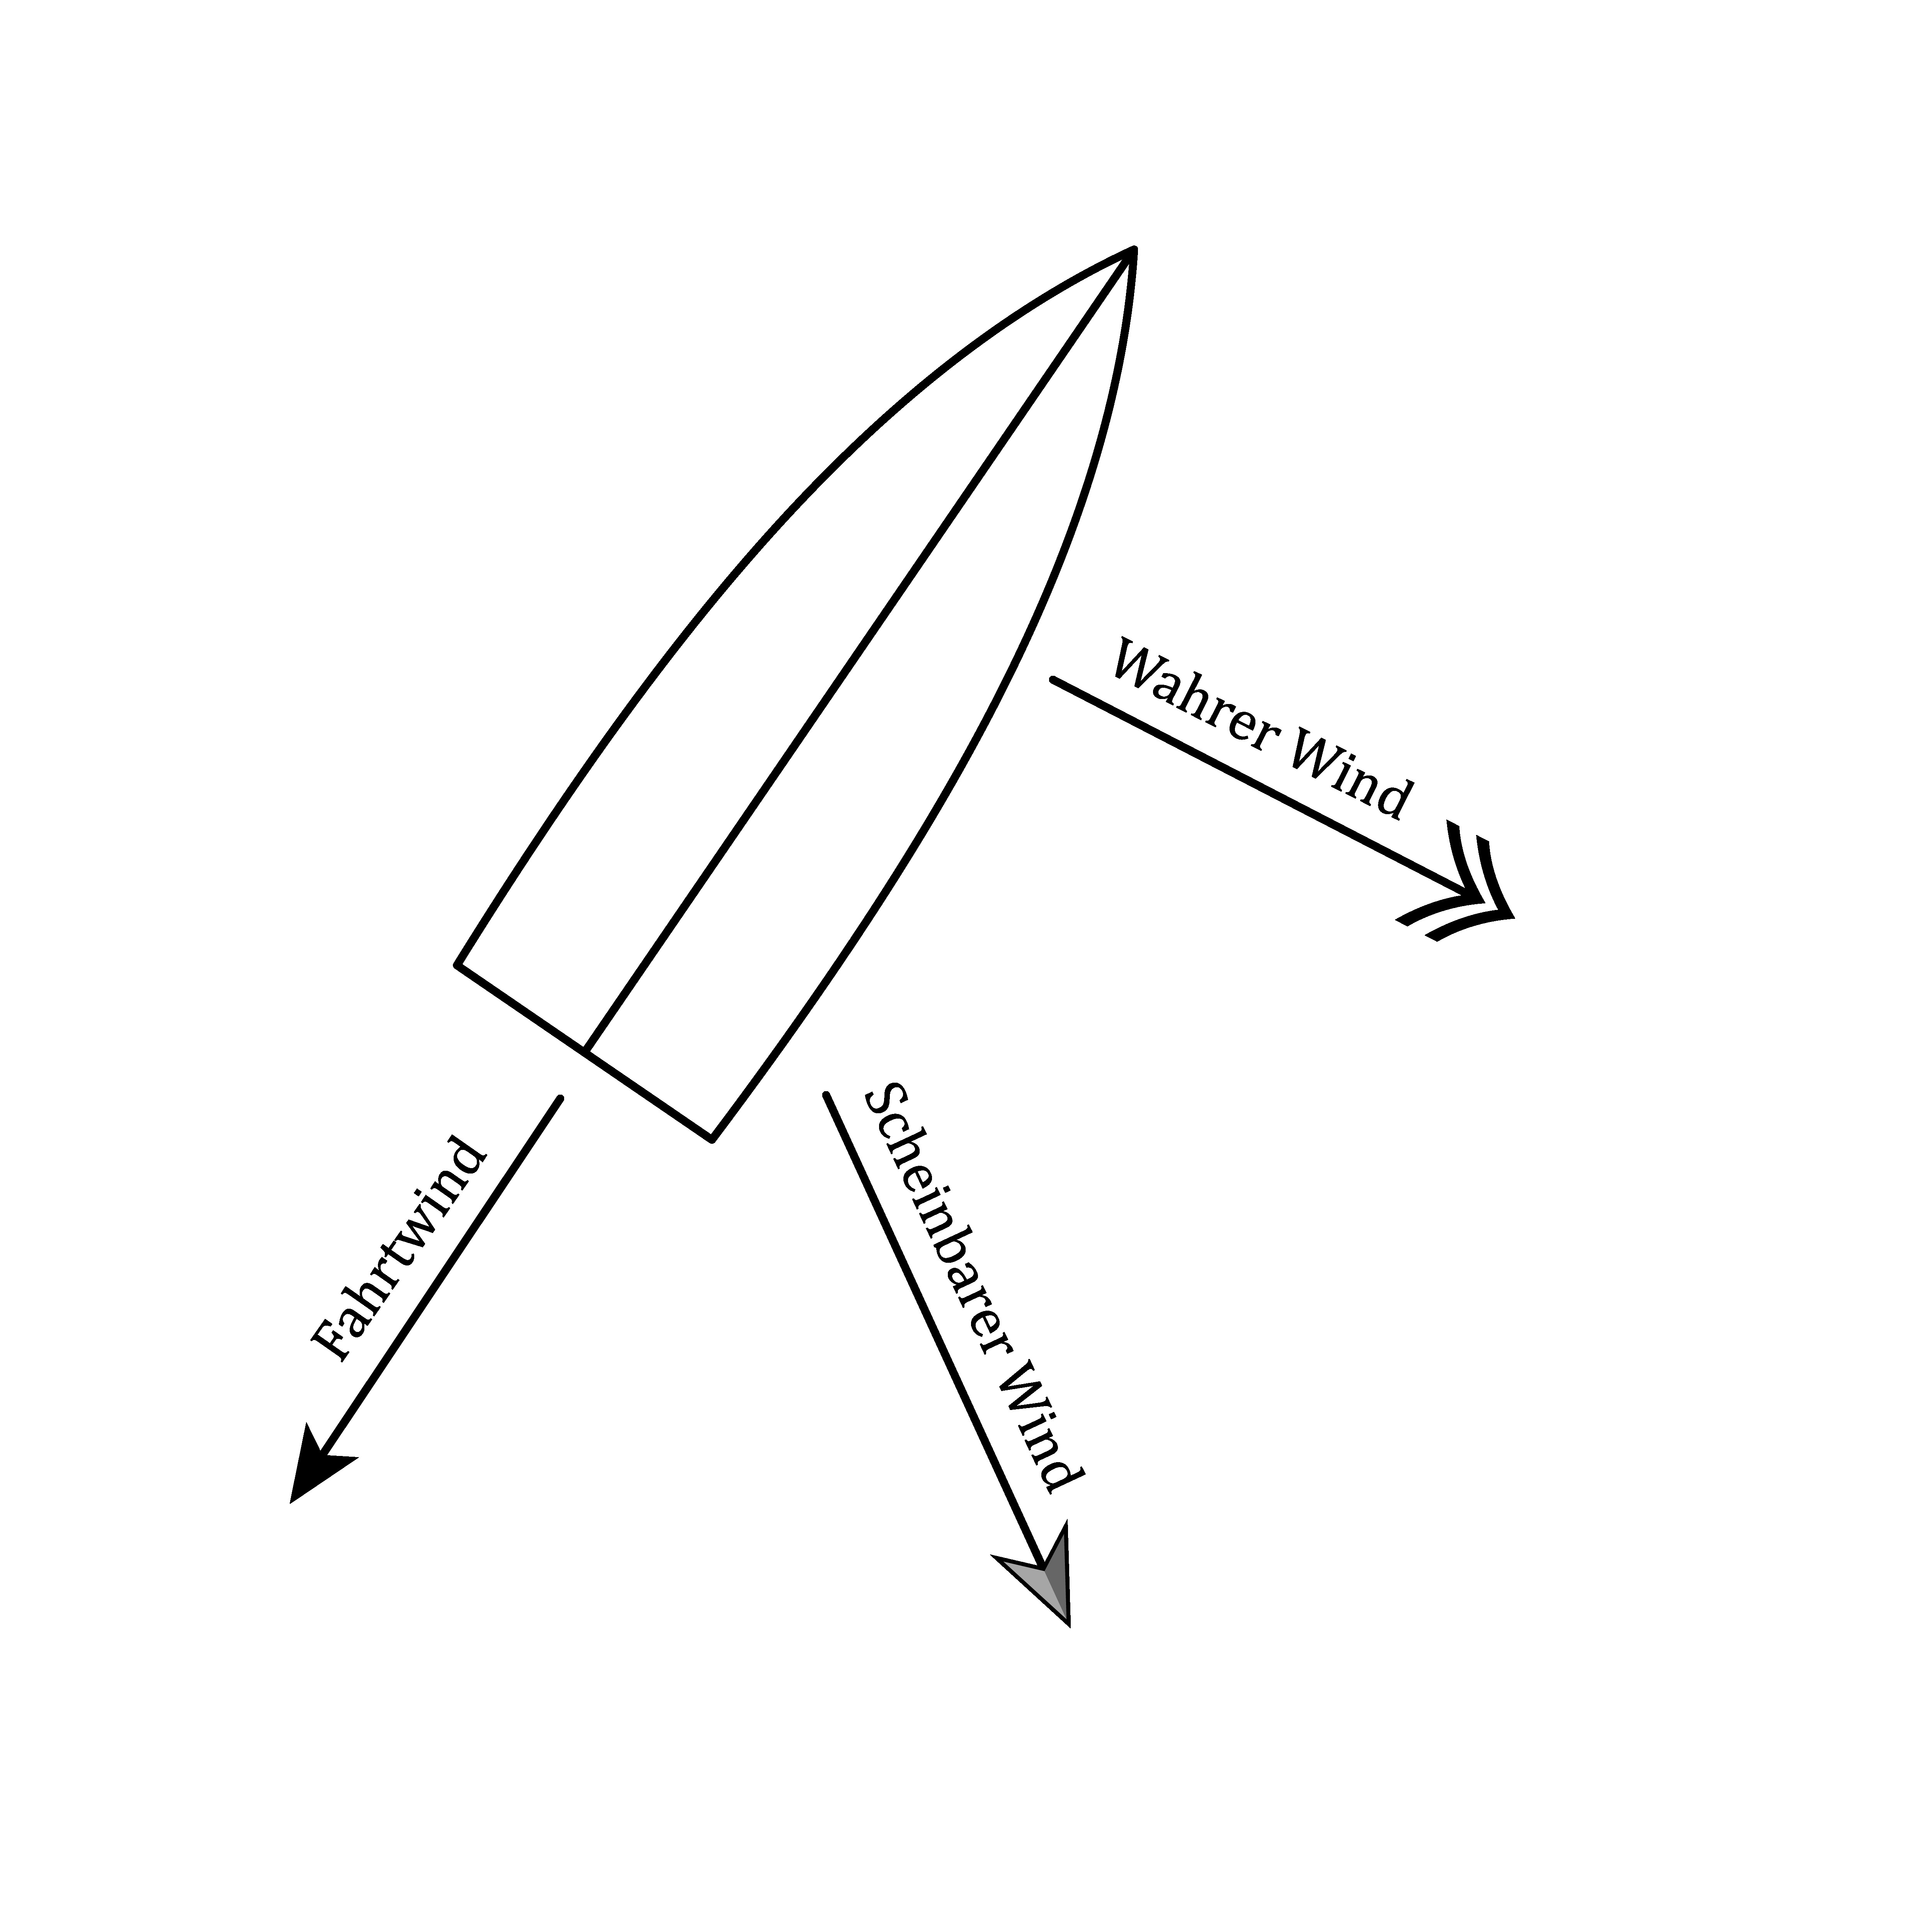
\includegraphics[width=0.75\linewidth]{assets/scheinbarerwind.png}
    \caption{Vektordarstellung des Windes}
    
\end{figure}

\section{Software}
\subsection{Programmiersprache}
Aufgrund der Anwendung auf einem ESP32 wurde das Program mit C++ entwickelt. In einer ersten Iteration ist Pyton auf einem Raspberry Pi gewählt worden. Aufgrund der mangelhaften Typisierung und der damit deutlich höheren Gefahr für Laufzeitfehler ist eine kompilierte Sprache hier angebracht. Ein Programmabsturz darf in einer solchen Anwendung nicht passieren weshalb die zuverlässigere Methode gewählt wird. 

Alternative Programmiersprachen wie Rust welche sich durch ihre Zuverlässigkeit auszeichnen haben eine deutlich kleinere Verbreitung.

Das Programm ist mit dem Arduino Framework und PlatformIO ertsellt worden. Dies vereinfacht das handhaben von mehreren Dateien und externen Bibliotheken.



\subsection{Aufbau der Software}
Die Architektur dieses Programms ist modular aufgebaut und besteht aus mehreren Klassen, die jeweils spezifische Aufgaben übernehmen. Die Hauptkomponenten sind:

\begin{itemize}
    \item \textbf{IMU}: Diese Klasse verwaltet die Inertial Measurement Unit (IMU) und stellt Methoden zur Initialisierung und Aktualisierung der Sensordaten bereit. Sie bietet auch Zugriff auf die Beschleunigungs-, Gyroskop- und Magnetometerdaten.
    \item \textbf{Actuator}: Diese Klasse steuert die Aktuatoren des Systems, insbesondere das Ruder und die Klappe. Sie bietet Methoden zur Initialisierung und Steuerung der Servos.
    \item \textbf{GPSManager}: Diese Klasse verwaltet das GPS-Modul und stellt Methoden zur Initialisierung und Aktualisierung der GPS-Daten bereit. Sie bietet auch Zugriff auf die aktuellen Positionsdaten, Höhe, Geschwindigkeit und Kurs.
    \item \textbf{BLEManager}: Diese Klasse verwaltet die Bluetooth Low Energy (BLE) Kommunikation. Sie initialisiert den BLE-Server und bietet Methoden zur Aktualisierung und Benachrichtigung von BLE-Charakteristiken.
    \item \textbf{Navigation}: Diese Klasse implementiert die Navigationslogik des Systems. Sie berechnet den optimalen Kurs basierend auf den aktuellen Positions- und Winddaten und steuert die Aktuatoren entsprechend.
\end{itemize}

Die Hauptlogik des Programms befindet sich in der \texttt{setup()} und \texttt{loop()} Funktion in der \texttt{main.cpp} Datei. In der \texttt{setup()} Funktion werden die verschiedenen Komponenten initialisiert, während in der \texttt{loop()} Funktion die Sensordaten regelmässig aktualisiert und die Navigationslogik ausgeführt wird. Die Kommunikation zwischen den Komponenten erfolgt über Singleton-Instanzen, die den Zugriff auf die jeweiligen Klassenmethoden ermöglichen.
Singleton wird gewählt, da somit ein Objektorientierter Ansatz auch für konkrete "Objekte" genutzt werden kann. Es ist somit aus der Programmstruktur klar, dass es nur ein spezifisches GPS Modul gibt.


\section{Webinterface für die Steuerung und das Monitoring des Segelboots}

\begin{figure}[H]
    \centering
    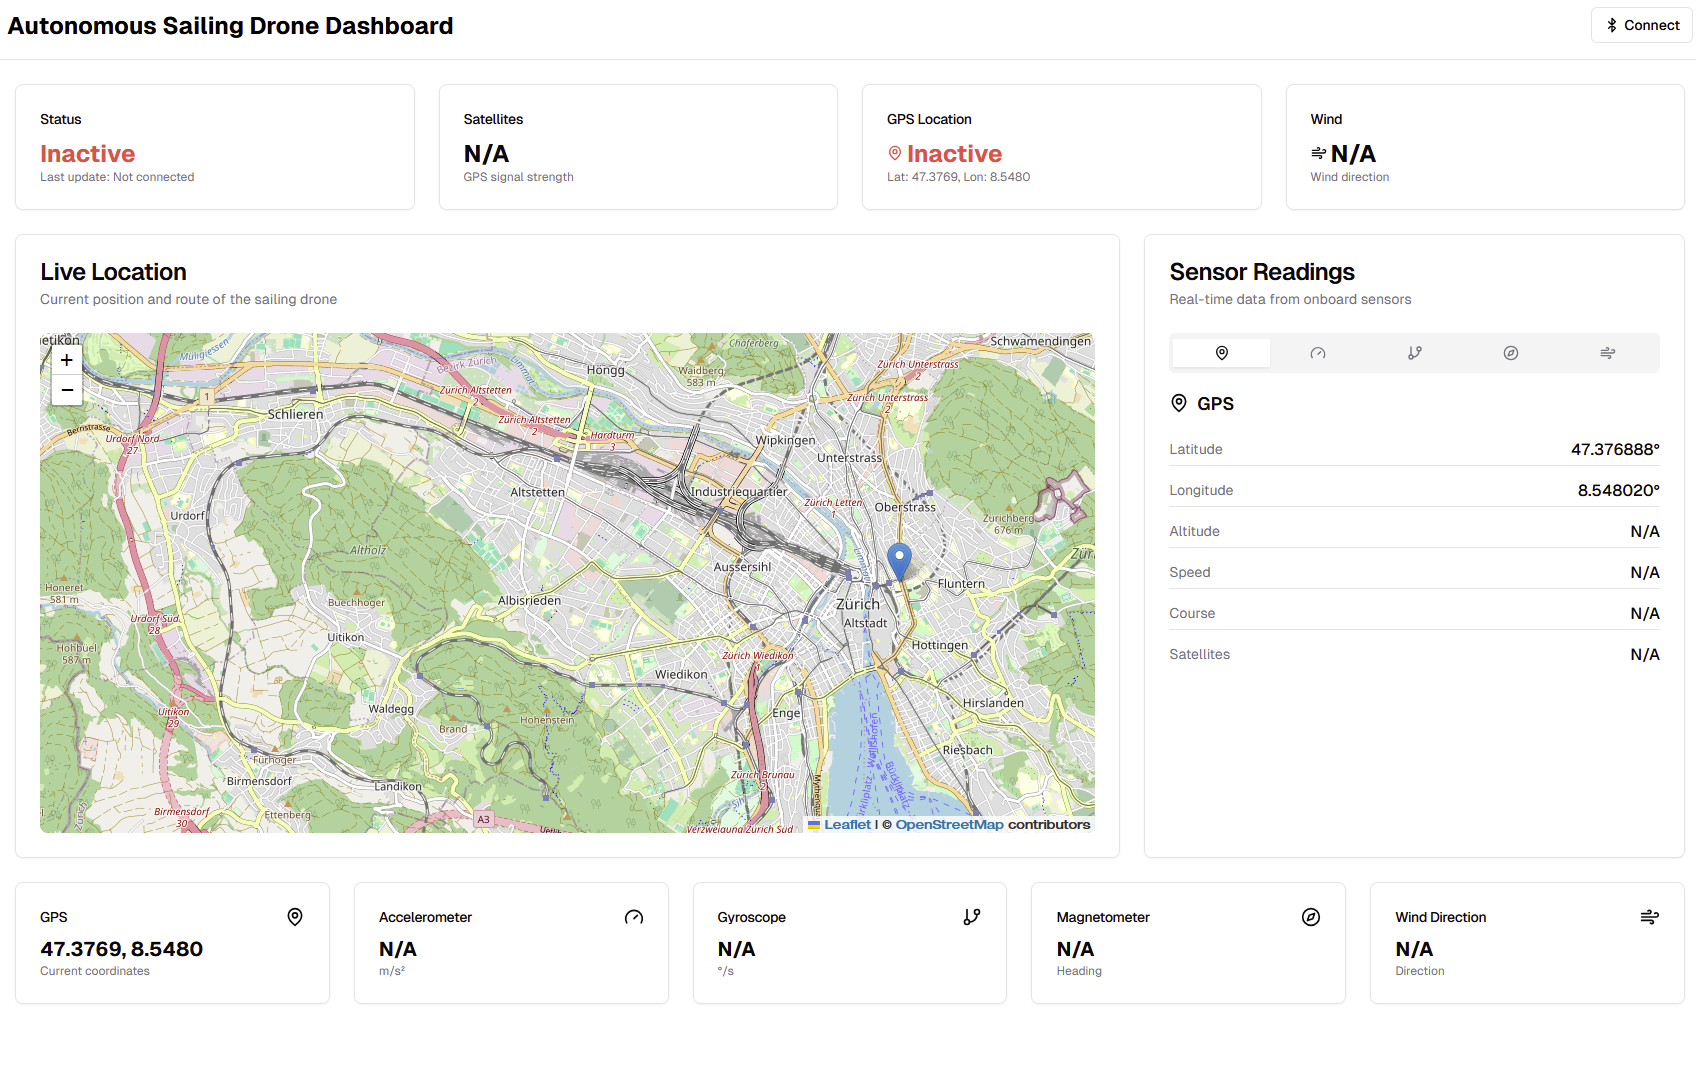
\includegraphics[width=1\linewidth]{assets/not cconnected interface.png}
    \caption{Dashboard (nicht aktiv)}
    \label{fig:enter-label}
\end{figure}

Um die Messwerte des Segelboots zu erhalten und dem Segelboot aus Distanz sein Ziel vorzugeben, wird ein Webinterface entwickelt. Diese macht sich die noch nicht weitverbreitete Implementierung der Web Bluetooth API zunutze. 

Das Segelboot verfügt über die Möglichkeit Daten über Bluetooth Low Energy (BLE) zu versenden. Dies ist, wie der Name bereits sagt eine Energiesparende Kommunikationsmethode die derzeit vor allem in Smarthome oder diversen Geräten wie Kopfhörer oder Tastaturen verwendet wird. Die Datenmenge die ausgetauscht werden kann ist relativ gering. Verwendet wird der Standard 4.2 der mit maximal 800 kbps keine grossen Datenmengen transferieren kann. 

Da dies für die Sensordaten nicht benötigt wird, kann auf viel Datentransfer verzichtet werden.


Die Möglichkeit über den Browser auf BLE Geräte zuzugreifen ist nicht weit verbreitet. laut mozilla.org wird dies derzeit nur von Chrome und Edge unterstützt. Aber auch bei diesen Browsern müssen zuerst die experimentellen Funktionen in den Einstellungen aktiviert werden.

Die Eigenschaft ohne Installation zusätzlicher Hardware am Computer, wie das bei den gängigen 433MHz Modulen der Fall wäre oder den erheblich höheren Energiebedarf der WLAN hätte, überwiegt die Einfachheit und Energieeffizienz von BLE. 

Aus dem Dashboard können folgende Werte Abgelesen werden.

\textbf{GPS-Navigationsdaten}
Die Positionsbestimmung erfolgt mittels eines satellitengestützten Navigationssystems mit folgenden Messgrössen:
\begin{itemize}
    \item \textbf{Breitengrad ($\varphi$):} Angabe in Dezimalgrad mit einer Präzision von $10^{-6}$ Grad
    \item \textbf{Längengrad ($\lambda$):} Angabe in Dezimalgrad mit einer Präzision von $10^{-6}$ Grad
    \item \textbf{Höhe ($h$):} Höhe über dem Meeresspiegel in Metern [m]
    \item \textbf{Geschwindigkeit ($v$):} Fortbewegungsgeschwindigkeit in Knoten [kn]
    \item \textbf{Kurs ($\alpha$):} Bewegungsrichtung in Grad [°] relativ zu geographisch Nord
    \item \textbf{Satellitenanzahl ($n_{\text{sat}}$):} Anzahl der empfangenen Satelliten zur Qualitätsbeurteilung des GPS-Signals
\end{itemize}

Die Signalqualität wird visuell durch Farbkodierung dargestellt: rot (inaktiv) bei $n_{\text{sat}} = 0$, gelb (eingeschränkt) bei $n_{\text{sat}} < 5$ und grün (aktiv) bei $n_{\text{sat}} \geq 5$.

\textbf{Beschleunigungssensor}
Der triaxiale Beschleunigungssensor erfasst die Beschleunigung in allen drei Raumrichtungen:
\begin{itemize}
    \item \textbf{X-Achse ($a_x$):} Beschleunigung in Längsrichtung in $\text{m}/\text{s}^2$
    \item \textbf{Y-Achse ($a_y$):} Beschleunigung in Querrichtung in $\text{m}/\text{s}^2$
    \item \textbf{Z-Achse ($a_z$):} Beschleunigung in Vertikalrichtung in $\text{m}/\text{s}^2$
\end{itemize}

\textbf{Gyroskop}
Das Gyroskop misst die Winkelgeschwindigkeit um die drei Raumachsen:
\begin{itemize}
    \item \textbf{X-Achse ($\omega_x$):} Rollrate in Grad pro Sekunde [°/s]
    \item \textbf{Y-Achse ($\omega_y$):} Nickrate in Grad pro Sekunde [°/s]
    \item \textbf{Z-Achse ($\omega_z$):} Gierrate in Grad pro Sekunde [°/s]
\end{itemize}

\textbf{Magnetometer}
Das Magnetometer dient zur Bestimmung der Ausrichtung relativ zum Erdmagnetfeld:
\begin{itemize}
    \item \textbf{Kurswinkel ($\psi$):} Ausrichtung in Grad [°] relativ zu magnetisch Nord
\end{itemize}

\textbf{Anemometer}
Der Windsensor liefert Daten zur Windcharakteristik:
\begin{itemize}
    \item \textbf{Windrichtung ($\theta_w$):} Richtung in Grad [°], aus der der Wind kommt
\end{itemize}

\textbf{Systemstatus}
Zusätzlich zu den Sensorwerten werden folgende Systemparameter überwacht:
\begin{itemize}
    \item \textbf{Verbindungsstatus:} Aktiv/Inaktiv je nach Bluetooth-Verbindungszustand
    \item \textbf{Letzte Aktualisierung:} Zeitstempel der letzten empfangenen Daten
\end{itemize}


Das Dashboard ist mit React und NextJs Entwickelt und verwendet die Ui Bibliothek von Vercel. Die Grundstruktur der Webseite wurde mit dem Ki Tool v0, welches ebenfalls von Vercel ist, generiert.





\section{Verbreitete Wegfindungsalgorithmen}
Für dieses Projekt wurden verschiedene Algorithmen auf ihre Eignung für dieses Projekt untersucht.

\subsection{Deep Reinforcement Learning Algorithm }
Deep Reinforcement learning ist ein Algorithmus aus der Familie des maschinellen Lernens. Seine Besonderheit ist, dass er im Gegensatz zum gewöhnlichen maschinellen Lernen keine Trainingsdaten benötigt. Hingegen wird ein \enquote{Agent} (vorliegend wäre das Segelboot der Agent) in eine virtuelle Umgebung gesetzt, in welcher er ein Ziel erreichen muss und dabei definierte Freiheitsgrade zur Bewegung hat. Wenn der Agent einen Fortschritt macht, wird dies belohnt. Macht er einen Fehler, wird er bestraft.

Der Nachteil dieses Algorithmus ist, dass er sich ausserhalb seiner trainierten Umgebung nicht zurechtfindet und dass die Bewegungen eines Segelboots sehr schwer in einer virtuellen Umgebung simuliert werden können. Eine auch nur ansatzweise akkurate Simulation würde den Rahmen dieser Arbeit eindeutig sprengen.
\subsection{Künstliche Potenzialfelder Algorithmus} 
Der Algorithmus der künstlichen Potenzialfelder ist eine Methode zur Pfadfindung, welche in der Robotik verbreitet ist. Der Algorithmus ermöglicht es, einen Weg zu finden, indem er auf anziehende und abstossende Felder reagiert, ähnlich wie dies in der Physik mit elektrischen Feldern geschieht.

Das Ziel des Algorithmus ist es, eine Richtung zu finden, in welche das Boot fahren soll, um vom Ausgangspunkt zu einem Zielpunkt zu gelangen. Dabei übt der Zielpunkt eine anziehende Kraft auf das Objekt aus, während Hindernisse eine abstossendend wirken entfalten. Mathematisch kann dies als Gradient dargestellt werden, bei dem die anziehende Kraft einen negativen Gradienten aufzeigt, der das Objekt zum Ziel zieht und die abstossende Kraft einen positiven Gradienten erzeugt, der das Objekt von Hindernissen abstösst.

Der gravierende Nachteil dieses Ansatzes ist, dass er in lokalen Minima stecken bleiben kann und tatsächlich auch stecken bleib. Überprüft wurde die Eignung des Ansatzes im Papier \enquote{Line following for an autonomous sailboat using potential fields method} \cite{inproceedings} . Dabei hat er sich auf offene Gewässer zwar als effizient erweisen, für engere Gewässer jedoch als ungünstig herausstellt.
\subsection{Vektor basierter Ansatz}


Die meisten der bekannten Algorithmen wurde mit Blick auf eine Überquerung
von Ozeanen oder die Navigation auf grossen Gewässern entwickelt. Dabei
spielen die Berücksichtigung von Wetterdaten etc. bei der Routenplanung
eine grosse Rolle. Für das vorliegende Projekt sind solche Thema aber nicht
relevant.
Es ist deshalb angezeigt, für das vorliegende Projekt einen eigenen Algorith-
mus zu entwickelt. Dieser basiert auf den Grundlagen der linearen Algebra
und lässt sich somit mit Gymnasialmathematik beschreiben. Ähnlich wie
beim Algorithmus der künstlichen Potenzialfelder wird bei jeder Berech-
nungsiteration der Kurs neu berechnet. Der Algorithmus hat eine gewisse
Ähnlichkeit zu demjenigen, welcher in A Simple Controller for Line Follo-
wing of Sailboats” beschrieben wird. \cite{sauze_simple_2013} Der Ansatz ist jedoch ganz anders
gewählt, daher ist die Ähnlichkeit vor allem in der Einfachheit. 


Der zentrale Algorithmus wird in der Methode \texttt{navigation\_step()} implementiert. Er wird in regelmässigen Abständen aufgerufen und entscheidet, wie das Boot seinen Kurs anpasst, um effizient zum nächsten Zielpunkt zu navigieren.

\subsubsection*{1. Vorbereitung der Daten}

Zunächst werden aktuelle Umgebungsdaten abgefragt:

\begin{itemize}
    \item \texttt{goal}: Zielposition als zweidimensionaler Vektor $(x, y)$, bestehend aus Längengrad und Breitengrad.
    \item \texttt{winddir}: Windrichtung in Grad, umgewandelt in Radiant.
    \item \texttt{currentHeading}: Kursrichtung des Bootes in Radiant.
\end{itemize}

Ausserdem wird die aktuelle Position des Bootes mit dem GPS abgefragt und als Vektor \texttt{currentPos} gespeichert.

\subsubsection*{2. Zielerreichung prüfen}

Das Boot überprüft, ob es sich bereits innerhalb eines Radius von 5 Metern um das Ziel befindet:
\[
\|\text{goal} - \text{currentPos}\| < 5
\]
Falls ja, werden Ruder und Flap auf neutral gesetzt.

\subsubsection*{3. Koordinatentransformation}

Die Windrichtung wird zunächst in ein lokales Koordinatensystem des Bootes transformiert. Dies erfolgt durch Anwendung einer Rotationsmatrix $R(\theta)$ mit dem Winkel des aktuellen Bootskurses:

\[
R(\theta) = 
\begin{bmatrix}
\cos(\theta) & -\sin(\theta) \\
\sin(\theta) & \cos(\theta)
\end{bmatrix}
\]

Die Transformation eines globalen Richtungsvektors (z. B. Windrichtung) in das Bootskoordinatensystem erfolgt durch:
\[
\vec{v}_{\text{lokal}} = R(\theta) \cdot \vec{v}_{\text{global}}
\]

So wird aus dem globalen Windvektor der relative Wind im Bootskoordinatensystem berechnet:
\[
\vec{v}_{\text{Wind,rel}} = R(\theta) \cdot \begin{bmatrix}\sin(\text{winddir}) \\ \cos(\text{winddir})\end{bmatrix}
\]

\subsubsection*{4. Prüfung auf Amwind}

Das Boot kann nicht direkt gegen den Wind segeln. Es prüft deshalb, ob der aktuelle Kurs in einem Bereich von ±45° zur Windrichtung liegt. Dies erfolgt durch das Skalarprodukt zweier normierter Vektoren:
\[
|\vec{v}_{\text{Boot}} \cdot \vec{v}_{\text{Wind,rel}}| < \cos(45^\circ) \approx 0{,}707
\]

Wenn diese Bedingung erfüllt ist, bedeutet das: Das Boot steht zu stark im Wind und muss einen Amwindkurs segeln.

\subsubsection*{5. Berechnung von Alternativkursen}

Zwei mögliche Amwindkurse werden generiert, indem zur Windrichtung jeweils ±45° addiert werden:
\[
\vec{v}_{\text{Option1}} = R(\theta) \cdot 
\begin{bmatrix}
\sin(\text{winddir} + 45^\circ) \\
\cos(\text{winddir} + 45^\circ)
\end{bmatrix}
\]
\[
\vec{v}_{\text{Option2}} = R(\theta) \cdot 
\begin{bmatrix}
\sin(\text{winddir} - 45^\circ) \\
\cos(\text{winddir} - 45^\circ)
\end{bmatrix}
\]

Diese Vektoren stellen mögliche Kurse dar, die den Wind in einem günstigen Winkel nutzen.

\subsubsection*{6. Auswahl des besseren Kurses}

Beide Kursoptionen werden mit dem Zielvektor verglichen, um zu bestimmen, welche Richtung effektiver ist. Hierfür wird wieder das Skalarprodukt verwendet:
\[
(\vec{v}_{\text{Ziel}} \cdot \vec{v}_{\text{Option1}}) 
\quad \text{vs.} \quad
(\vec{v}_{\text{Ziel}} \cdot \vec{v}_{\text{Option2}})
\]
Der Vektor mit dem höheren Wert zeigt stärker in Richtung des Zieles und wird daher gewählt.


\section{Kollisionsvermeidung}
Damit das Segelboot nicht auf Grund läuft, muss es über eine Funktion zur Kollisionsvermeidung verfügen. Diese funktioniert jedoch nur mit vorher einprogrammierten Hindernissen wie dem Ufer, Inseln, Sandbänken oder Naturschutzgebieten. 

Dabei wird dasselbe Prinzip angewendet wie dem Aufkreuzen (gegen den Wind fahren). Dabei wird bei jeder Iteration die Distanz zu den Hindernissen berechnet. Falls diese geringer als 40 m ist, erkennt das Boot diese als Gefahr und weicht ihnen aus.  

Hindernisse werden immer als Punkt behandelt. Grosse Hindernisse wie Inseln oder das Ufer müssen als eine Vielzahl von Punkten vorgegeben werden. Sobald Hindernisse in der unmittelbaren Nähe (40 m) des Bootes sind, erfährt die übliche Navigation die folgende Modifikation.

Als erstes werden die Vektoren zwischen den Hindernissen und dem Boot in einer Liste gespeichert. Beim Berechnen der neuen Richtung wird nun nicht mehr nur das Skalarprodukt zwischen dem Wind und dem Boot in Betracht gezogen, sondern ebenfalls das Skalarprodukt zwischen den einzelnen Hindernissen und dem Boot. So wird dann versucht, eine neue Richtung zu finden.

Die Nachteile dieses reaktiven Ansatzes sind offensichtlich. Das Boot könnte allenfalls in engen Buchten gefangen bleiben, weil es kein Weg aus diesen findet. Dies lässt sich aber dadurch vermeiden, dass dem Boot die Einfahrt in die Bucht durch ein entsprechendes Ziehen der Uferlinie grundsätzlich untersagt wird. 
\section{Motorsteuerung}
Wie im Kapitel Elektronik bereits ausgeführt, werden zwei Aktuatoren verwendet. Beide können mit einen einzigen 5 V Steuerimpuls in die eine gewünschte Position bewegt werden, wobei die genaue Position durch die Dauer des Impulses (zwischen 1 ms und 2 ms) bestimmt wird. 
\subsection{Ruder (PID Controller)}
Für das Ruder des Segelboots ist ein Regelungssystem notwendig, damit das Boot in die richtige Richtung gelenkt wird. Hierfür wird ein PD Controller verwendet. Der Name \enquote{PD} steht für Proportional (P) und Derivative (D). Diese Begriffe beschreiben die Hauptkomponenten des Regelungsalgorithmus. Der proportionale Teil des Reglers misst den Fehler zwischen der aktuellen Ausrichtung (des Bootes) und der gewünschten Ausrichtung. Dieser Fehler wird als Vektor dargestellt. Der P-Anteil multipliziert diesen Fehler mit dem Verstärkungsfaktor (Kp), um einen ersten Korrekturwert zu generieren. Demnach gilt, je grösser der Fehler ist, desto grösser muss die Korrektur sein. Mit diesem Teil des Reglers wird das Ruder erstmals in die richtige Richtung gelenkt. Der Derivativteil (D) des Reglers achtet darauf, wie sich die Änderung des Fehlers verhält. Wenn das Boot sich dem gewünschten Kurs nähert, kann der Fehler schnell abnehmen, was zu einem Überschwingen führen kann. Der D-Teil versucht, dieses Überschwingen möglichst zu reduzieren, indem er den Fehlergeschwindigkeitsvektor (sprich die Ableitung des Fehlers) berechnet. Dieser wird ebenfalls mit einem Verstärkungsfaktor multipliziert. Aus der Kombination von P- und D-Komponenten kann eine Ruderposition, die zwischen 0 und 1 liegt, berechnet werden. Ein Wert von 0.5 entspricht dem Ruder, welches sich, wenn alles stimmt, in der Mitte befinden sollte. Somit kann sich das Boot sanft an den gewünschten Kurs annähern, ohne dauernd zu übersteuern. 
\subsection{Segel}
Da das Segel kann wie im Abschnitt \ref{sec:sailflap} \nameref{sec:sailflap} bewegt werden. Da die Schnelligkeit des Bootes bei dieser Arbeit untergeordnet ist, wird das Sailflap immer in die Richtung des Windes gedreht. Dies sorgt dafür, dass das Segel in eine segelbare Position geführt wird. Diese wird in den meisten Fällen nicht optimal sein  jedoch ausreichend für diesen Anwendungsfall.
\begin{figure}
    \centering
    \includegraphics[width=0.75\linewidth]{sailflap_erklärung.png}
    \caption{Sailflap Visualisierung}
    \label{fig:enter-label}
\end{figure}